\section*{Capturing physical, technical and economic constraints on power generation: a description of the IMACLIM-R electricity nexus}

IMACLIM-R is a twelve region, recursive, hybrid general equilibrium model that includes a technology-rich, bottom-up energy sector.  The long term investment decision is represented by a multinomial logit structure in which 20 explicit technologies compete based on the most up-to-date electricity generation costs. The cost competition takes place under imperfect foresight and with different possible regimes of beliefs about future climate policy. The key features of the electricity supply are represented: capital vintaging, fuel efficiency, utilization rate, carbon capture and storage, renewable energy integration challenges.  Both investment and dispatch decisions are made on an annual basis, from the model's base year (2014) to 2100 to provide meaningful insights into future electricity systems, their contribution to climate change mitigation and their linkages with the rest of the economy.

\begin{figure}[H]
    \centerline{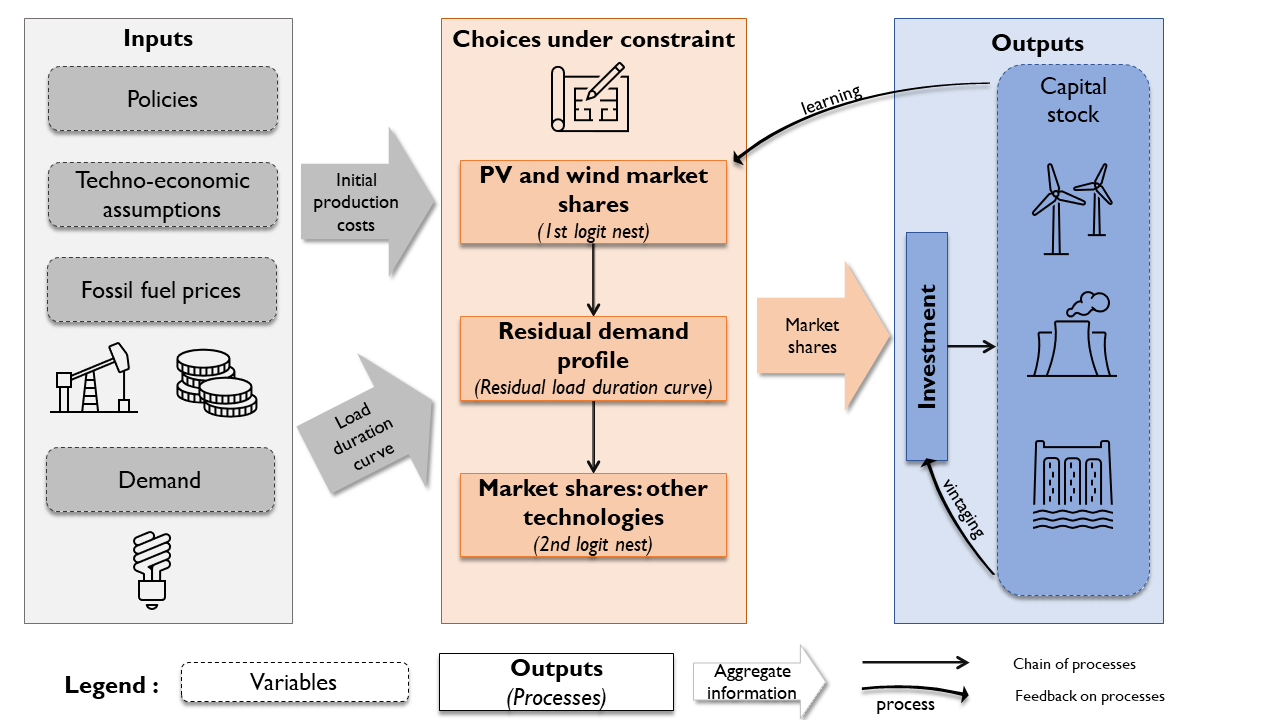
\includegraphics[scale=0.55]{figures&tables/Summary_nexus.png}} %not bad for centering!!
    \caption{Summary of the investment procedure in the power sector}
    \label{fig:suminv}
\end{figure}

\section{Introduction}
The electricity sector is receiving special attention under the low-carbon transition, as it is a massive lever for reducing greenhouse gas (GHG) emissions. Electricity generation accounted for 44\% of global CO2 emissions in 2019. Climate change mitigation undoubtedly goes hand in hand with a technological shift to renewable energy. In fact, the emissions of the electricity sector come from the combustion of fossil resources, namely coal, oil and gas, in existing power plants. Given the inertia of capital in this sector (power plants are expected to operate for decades), today's option for electricity generation are determined by the capacity built in the past. Therefore, an accurate representation of power capacity investment decisions is key to capturing current and future developments in the electricity sector.


Ultimately, representing the key features of electricity systems imposes that two types of decisions made under techno-economic constraints are considered:
\begin{enumerate}
    \item the long-term choice of optimal capacity to meet future electricity demand
    \item the short-term choice of capacity utilization to meet current load (dispatch).
\end{enumerate}

We cover these two decisions in the four next sections. \textbf{Section 2} describes the technical and cost assumptions underlying the choices of electricity generation capacities. \textbf{Section 3} presents the inclusion of the load curve constraint. \textbf{Section 4} details the investment process, characterized as optimal planning of investments under imperfect foresight. \textbf{Section 5} describes the dispatch decision. The last two sections details the linkages between the electricity nexus and the rest of the economy (\textbf{Section 6}) while (\textbf{Section 6}) presents the key outputs of the nexus.

\section{Explicit electricity generation technologies described in terms of capital generation}

\paragraph{ Cost assumptions and technical change in the electricity sector}

The description of the electricity generation mix is based on a discrete set of  21  technologies. Each of the  21  technologies is characterized by a set of techno-economic parameters that allow its levelized cost of electricity (LCOE) to be computed. These parameters include: investment costs ( in \$ per \kw  installed), energy efficiency ($rho$, in \% for the technologies using fossil fuels), fixed and variable operation and maintenance costs (\$ per \kw installed and \$ per \kwh produced), , an availability factor for dispatchable technologies (in \% of full load hours), a capacity factor for non-dispatchable technologies (in \% of full load hours), lifetimes, and a discount rate (in \%) that includes both the opportunity cost of capital and a unique risk factor for each technology.

The techno-economic parameters for each technology are calibrated using sectoral technology models or information from the literature (%\cite{IEA2020}, \cite{IRENA2020}).
For technologies that are scaled up or developed, costs decrease over time through a global learning process modeled by learning curves (\cite{Neij2008}). Learning curves link production costs to cumulative production through a learning coefficient. In the case of the electricity sector, the cost of electricity production is expected to decrease with cumulative installed capacity for a given technology. In the base year of the model (2014), all regions in the IMACLIM-R model start with different cost assumptions. In addition, floor costs are defined in each region: these are the lowest costs that can be achieved through a learning process. As a result, the learning process is global (every region benefits from other's capacity additions) but the initial and asymptotic costs remain differentiated (or can be). This choice is motivated by two findings: 1) wind turbines and PV modules being traded as a commodity 2) persisting capital costs differences depending on the location, due to national or regional context such as labor costs. With $CINV \textunderscore MW\textunderscore nexus\textunderscore {k,j}(t)$ the current investment cost for technology $j$ in region $k$ at time $t$, $CINV\textunderscore MW\textunderscore nexus \textunderscore ref_{k,j}$, the reference investment cost (at calibration year), $A\textunderscore CINV\textunderscore MW\textunderscore ITC\textunderscore ref_{k,j}$ the floor cost,  $LR\textunderscore ITC\textunderscore elec_{j}$ the learning rate, $Cum\textunderscore Inv\textunderscore MW_ elec_ ref_{k,j}$ the cumulated investment of technology $j$ in region $k$ at calibration year, $Cum\textunderscore Inv\textunderscore MW\textunderscore elec_{k,j}(t)$ the cumulated investment at time $t$:

\begin{dmath}
    CINV\_MW\_nexus_{k,j}(t) = max(A\_CINV\_MW\_ITC\_ref_{k,j},CINV\_MW\_nexus \_ref_{k,j}*(1-LR\_ ITC\_elec_{j})^{log(\frac{Cum\_Inv\_MW\_elec_{k,j}}{Cum\_Inv\_MW_elec_ ref_{k,j}})})
    \label{eqn:LR}
\end{dmath}

Moreover, as renewable energy costs have declined recently, the CAPEX and OPEX curves for wind and solar (including CSP) are driven to match recently observed values in the region. It means that between 2014 and 2019, the decline in renewable costs is monitored and not driven by the learning curve.

\paragraph{ Carbon Capture and Storage }
The electricity nexus of IMACLIM-R includes both fossil fuel carbon capture and storage (CCS) and bioenergy with CCS (BECCS) technologies. In the current version of the model, CCS for power generation technologies does not enter the R\&D stage until a threshold for the current regional carbon price is reached to prevent early CCS deployment despite low or negative profitability. The market share of each CCS technology is limited by an S-shaped technology development function. In the case of BECCS, an additional biomass supply curve (\cite{Hoogwijk2009}) limits the deployment of this technology. In the current structure of IMACLIM-R, BECCS are the only source of negative emissions. Therefore, the pace of BECCS deployment is critical in very low-carbon/net-zero mitigation pathways. Fossil fuel technologies are not allowed to be retrofitted with CCS, so new power plants must be built to capture and store carbon.


\paragraph{ Capital inertia }
In the electricity sector, the capital stock is path-dependent, because each investment at time t adds to the capacity built in previous periods. The variable $Cap\textunderscore elec\textunderscore MW\textunderscore vintage_{k,j}(t)$ tracks down yearly capacity additions for technology $j$ in region $k$. Thus, the depreciated capital at the time $t$ is the sum of the capital generations reaching the end of their lifetime from the time $t - lifetime$ to $t - 1$. When adding the new investment to the depreciated stock of capital at time t, one gets the functionning capital at time t before the new capacity addition from investment.
\begin{dmath}
    Cap\_elec\_ MW\_vintage_{k,j}(t) = Inv\_MW_{k,j}(t)
    \label{eqn:Cap_elec_vintage}
\end{dmath}

\begin{dmath}
    Cap\_elec\_MW\_dep_{k,j}(t) = \sum_{i = t - lifetime_{k}}^{t-1}Cap\_elec\_MW\_vintage_{k,j}(i)
    \label{eqn:Cap_elec_dep}
\end{dmath}

\begin{dmath}
    Cap\_elec\_MW_{k,j}(t) = Cap\_elec\_MW\_dep_{k,j}(t) + Inv\_MW_{k,j}(t)
    \label{eqn:Cap_elec}
\end{dmath}





At each time step of the model, the average characteristics of the installed production capacity are the weighted average of the technical characteristics of the different generations of power plants still in operation.
The inertia of plants and the embodied nature of technologies are represented by tracking capital across generations along with technological characteristics.


Every year, the production units that reach the end of their lifetimes are retired.
Adding the annual capacity additions $i.e.$ investments, we obtain a net installed production capacity.

The new generation of capital capacity and its technological characteristics are determined by investment choices, represented as described in the following sections.


\section{A challenge to incorporate demand-side and renewable energy supply constraints in a compact electricity module}

\paragraph{Final energy demand in IMACLIM-R}
In IMACLIM-R, the final energy demand arises from three (meta) sectors: the productive sectors, the transportation sector and the residential sector. For the transportation and the residential sectors that benefit from detailed bottom-up representations, the use of electricity depends on explicit technology choices, $e.g.$ purchasing electric cars rather than thermal ones. In the case of productive sectors (agriculture, industry, construction, composite good), the electricity demand is determined by input-outputs coefficients.

\paragraph{The load duration curve}

To model investments in the electricity sector in a stylized way i.e., without coupling the macroeconomic core of IMACLIM-R with a high-resolution energy model, it is common to combine the daily load curves over the 365 days of the year into a single curve called the load duration curve.
The load duration curve is obtained by plotting the hourly load values over the year against the duration for which that load was requested. The highest recorded load over the 8760 hours of the year is called the peak load. The minimum power supplied throughout the year is the base load. This way, the balance between electricity demand and supply can be solved annually.


The shape of the load duration curve is specific to each region, as it is directly related to the temporal variability of electricity demand. In particular, this variability depends on the seasonal climate variations in the region
For numerical simplicity, the regional load duration curves have been approximated by segmented linear functions:
\begin{itemize}
    \item the possible annual loads (measured in hours) are divided into seven intervals with the following boundaries: [0, 730, 2190, 3650, 5110, 6570, 8030, 8760];
    \item the maximum load lasts 730 hours (peak load);
    \item the minimum load lasts 8760 hours (base load);
    \item the load level for the other periods of time is calculated by dividing the interval between baseload and peak load into six equal segments $i.e.$ 760 hours of baseload, 760 hours of peak load, and five segments in between of 1460 hours each.
\end{itemize}

Hence, the load duration curve shape on Figure \ref{fig:LDC}: one peak load band, 5 inner load bands and one baseload band.
Using this simplified scheme, the load duration curve of each region can be fully characterized by two values: peak load and baseload. The annual electricity produced is given by the surface under the curve presented in Figure \ref{fig:LDC}\footnote{In this Figure, the "real load duration curve" correspond to a hypothetical example, to highlight the way load duration curves are approximated. The reader should keep in mind that there is no such "real load duration curve" in IMACLIM-R, only an annual electricity demand from which an approximated load curve is derived}.

\begin{figure}
    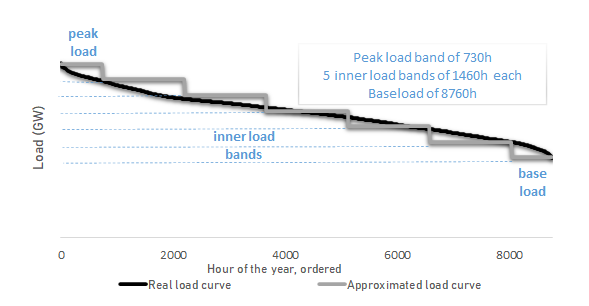
\includegraphics{figures&tables/LDC.png}
    \caption{Load duration curve approximation in IMACLIM-R's electricity module}
    \centering
    \label{fig:LDC}
\end{figure}


To calibrate and reconfigure the load duration curve for each time period, we assume that the ratio of peak load to baseload, (written $bp\_ratio_k$) remains constant and equal to a value supplied by the POLES model.\footnote{
    In principle, this ratio could vary in an exogenous or endogenous manner to integrate, for example, its modification under the effect of policies of demand side management. These policies are not implemented in the current version of the model.
}
The load duration curve approximation associated with a quantity $Q\_elec_k$ of electricity produced in the region $k$, is obtained by solving the equation system, formed by the ratio constancy equation and the constraint equation on the quantity of energy produced, as described in equations \ref{eqn:elecBpRatio} and  \ref{eqn:elecQ}
where $base_k$ and $peak_k$ are the loads required during the base or peak periods respectively.

\begin{dmath}
    \frac{base_k}{peak_k} = bp\_ratio_k
    \label{eqn:elecBpRatio}
\end{dmath}

\begin{dmath}
    Q\_elec_k =
    peak_k * 730 +
    base_k * 8760 + \frac{peak_k - base_k}{6} * ( 8030 + 6570 + 5110 + 3650 + 2190)
    \label{eqn:elecQ}
\end{dmath}

The load duration curve shape informs both about the optimal size of generating capacity required to meet peak demand and when to utilize this capacity throughout the year. To go further, we must account for the impact of renewable power over the load duration curve. Residual Load Duration Curves (RLDCs) encapsulate the physical and temporal constraints on electricity demand and supply, including the challenges to variable renewable energy integration into power systems.

\paragraph{The residual load duration curve and the challenges to VRE integration }

Variable renewable energy (VRE) sources such as solar PV or wind are intrinsically non-dispatchable. Thus, their deployment has an impact on the operation of power systems (\cite{Hirth2015}). VRE generation increases the need for flexibility of the power system, including dispatchable power to meet peak demand. Indeed, the capacity credit of VRE (the ability to contribute to peak demand in a power system) is low and decreases as the VRE share in the mix increases.

For technologies to compete on an equal footing (dispatchable vs variable), we first must correct VRE Levelized Cost of Electricity (LCOE) to account for its low capacity credit, $i.e.$ variable renewable energy sources contribution to meeting peak demand. In other words, the "hidden costs" associated with VRE generation are not included in VRE LCOE. Therefore, we add what we call "integration costs" to the VRE LCOE to calculate the System VRE LCOE system that covers the full economic costs of solar and wind generation. Integration costs measure the costs imposed on the electricity system to maintain the marginal value of renewable electricity. They include investments in storage facilities, grid costs, backup costs, etc. Typically, integration costs are divided into three categories, each related to the fundamental characteristics of renewables: Uncertainty, locational constraints, and variability.
\begin{itemize}
    \item Balancing costs (uncertainty). They gather actions taken to face VRE output unpredictability, for instance, the cost of intraday trading. Balancing costs tend to zero in absence of forecasting errors on VRE output.
    \item Grid-related costs (locational specificity). Grid-related costs measure the reduction in market value due to the specific generation location of power plants.
    \item Profile costs (variability). Profile costs reflect the marginal value of electricity at different moments in time. As the demand varies through time, profile costs measure the cost of matching this demand with VRE storage devices or conventional backup power.
\end{itemize}

However, estimating value ranges for profile costs and other integration costs is not straightforward. With 20\% renewables in the electricity mix, reported values for integration costs range from €0/MWh to €49.2/MWh, \cite{Heptonstall2021} reflecting a high degree of uncertainty in integration cost estimates. Indeed, the extent of the depreciation of renewable electricity depends on the (in)flexibility of the rest of the electricity system. The more flexible the system, the lower the integration costs. Consequently, estimates of integration costs depend on the underlying energy model and its techno-economic assumptions. Explicitly representing flexibility options such as V2G or P2G would have drastically increased the complexity of the power system and is beyond the scope of this module. Therefore, we chose a synthetic way to account for integration costs through an integration cost markup for PV and wind. The PV (resp. wind) markup, expressed in \$ per MWh of PV (resp. wind), is linear with respect to the share of wind and PV gross generation and sums to the PV (resp. wind) electricity production cost. The parameters $\alpha$, $\beta$, $\gamma$, and $\delta$ are calibrated to reflect typical values of integration costs (in \$ per MWh of VRE generation).

\begin{dmath}
    Markup^{pv}_k = \alpha * share\_pv_k + \beta * share\_wind_k
\end{dmath}
\begin{dmath}
    Markup^{wind}_k = \gamma * share\_pv_k + \delta * share\_wind_k
\end{dmath}
\begin{dmath}
    Integration\_costs_k = Markup^{pv}_k *
    \frac{share\_pv_k}{share\_pv_k + share\_wind_k} +
    Markup^{wind}_k * \frac{share\_wind_k}{share\_pv_k + share\_wind_k}
\end{dmath}

%plot the values of VRE

We still lack robust data to calibrate the integration cost markup parameter and we rely on the few existing study to do so. These parameters shall be updated as soon as comprehensive peer-reviewed studies on integration costs will be published. The sensibility analysis presented on Figure [coming: sensibility analysis on the markup parameters] show that the integration cost markup parameters are of great importance for VRE deployment.

The VRE markup is the counterpart of the cost of variable renewable energy sources on the rest of the electricity system. This is captured physically by a distortion of the residual load duration curve as the share of renewable energy in the mix increases: the higher the share of renewable energy, the steeper the residual load duration curve \cite{Ueckerdt2015}. Thus, following the ADVANCE project "Variable Renerwable Energy integration module" framework (\cite{Ueckerdt2017}), the residual peak load becomes a function of the VRE gross generation:

\begin{dmath}
    {peak\_res_{k}} = f(Gross\_wind\_share_{k},Gross\_pv\_share_{k})
    \label{eqn:peakres}
\end{dmath}
with the $f$ a third-order polynom (see Annex for the polynomial coefficients).


This way, $base\_res$ and $peak\_res$ are now determined by Equations \ref{eqn:peakres} and \ref{eqn:elecQres}: Equation \ref{eqn:elecBpRatio} no longer holds. However, Equations \ref{eqn:peakres} and \ref{eqn:elecQres} do not prevent negative residual baseload. Thus, Equation \ref{eqn:elecQres} includes the possibility to adapt if solving the system of equations \ref{eqn:peakres} and \ref{eqn:elecQres} yields negative residual baseload. If for  $nb\_steps$ = 6 (starting case), the residual baseload is negative, the 8760h load band is removed, and the system of equations \ref{eqn:peakres} and \ref{eqn:elecQres} is solved again with one less load band, as shown on Figure \ref{fig:RLDCapprox}. This way, the residual load curve is always positive and conserves its properties\footnote{A version of the residual load duration curve design with a miminum load band (\cite{Ueckerdt2015}) (continuous supply from dispatchable plants throughout the year) is currently under study}.

% adapted from doi: 10.1016/j.renene.2014.08.065 

\begin{dmath}
    Q\_elec\_res_k =
    {peak\_res_k} * 730 +
    {base\_res_k} * {lower\_load\_bands_k} +
    \frac{peak\_res_k - base\_res_k}{nb\_steps_k} * ( \sum inner\_load\_bands_k)
    \label{eqn:elecQres}
\end{dmath}


The residual peak load and the net share (without curtailment) of non-VRE generation in total demand depend on the gross VRE generation. Additionally, the ADVANCE project module was also used to calibrate 1) VRE curtailment and storage losses 2) storage capacity and output as a function of the share of solar PV and wind energy in the mix, the same way the residual peak load does (see equation \ref{eqn:peakres}).

\begin{dmath}
    {curt_{k}} = g(Gross\_wind\_share_{k},Gross\_pv\_share_{k})
    \label{eqn:curt}
\end{dmath}

\begin{dmath}
    {stor\_cap_{k}} = h(Gross\_wind\_share_{k},Gross\_pv\_share_{k})
    \label{eqn:stor_cap}
\end{dmath}

\begin{dmath}
    {stor\_output_{k}} = m(Gross\_wind\_share_{k},Gross\_pv\_share_{k})
    \label{eqn:stor_out}
\end{dmath}




%cite Ueckerdt, Pietzcker et al. from https://fp7-advance.eu/?q=content/variable-renewable-energy-integration-module
\begin{figure}[H]
    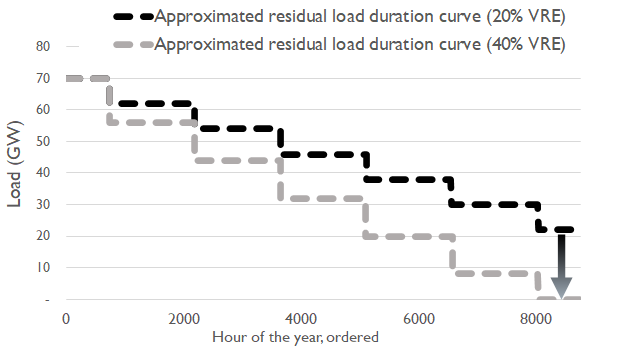
\includegraphics[scale=0.8]{figures&tables/LDC&RLDC.png}
    \centering
    \caption{Illustrative RLDC approximation for 20\% and 40\% net VRE share}
    \label{fig:RLDCapprox}
\end{figure}

In the end, this residual load duration curve design allows representing VRE integration challenges in a compact electricity module such as IMACLIM-R's by relying on the highly resolved Dispatch and Investment Model for Electricity Storage (DIMES)  outputs. Basically, it allows the electricity sector of IMACLIM-R to include the impact of variable renewable energy on the electricity system in a simple, yet robust manner. It captures key mechanisms behind the variable renewable energy penetration challenge and yields consistent results (see Figure X in Annex).

\paragraph*{Storage}
For now, only short-term storage is represented in the electricity nexus: storage capacity, outputs and losses are extracted from the DIMES output (see equation \ref{eqn:stor_cap} and \ref{eqn:stor_out}) and DIMES only optimizes short-term storage. Thus, seasonal (long-term) storage is not included yet in the electricity nexus.

\section{Optimal planning of investments under imperfect foresight}

With the compact representation of power generation technologies and the (residual) load duration curve presented above, we have the necessary technical details to model investment decisions in the power sector on an annual basis.
The investment decision can be described as a cost minimization procedure under imperfect foresight to meet future electricity demand under technological constraint. At each time step, the central planner of the electricity sector selects an ideal electricity mix to meet the projected demand at the short-term horizon (ten years by default), from which an annual investment plan is derived.
The decision procedure is decomposed into five successive steps:
\begin{enumerate}
    \item Formulating expectations about future demand and future fuel prices;
    \item Choosing  wind turbine and solar PV  electricity production capacity;
    \item Choosing hydroelectric production capacity;
    \item Projecting the optimal conventional (non-renewable) production capacity to meet domestic demand;
    \item Deciding on the annual investment increase necessary to move the existing production capacity towards the optimal capacity that has just been calculated
\end{enumerate}

Separating the treatment of VRE and hydroelectric energy is justified by the specificities of these energy sources. A more detailed explanation of these specificities is given below.

\paragraph{Projecting demand and anticipating fuel prices}

The optimal installed capacity and level of annual investments are determined using backward-looking expectations of electricity demand growth and  future fossil fuels prices over the coming ten years.

The regional projections of electricity production for the period $t+10$, written $Q\_elec_k^{anticip}$, are derived from the current annual growth rate of electricity production, $tendency_{Q\_elec_k}$, which is taken to be stable for the next ten years, and the current electricity production, $Q\_elec_k$ (in $MWh$).

\begin{dmath}
    Q\_elec_k^{anticip} = Q\_elec_k * \left( 1 + tendency_{Q\_elec_k}\right) ^{10}
    \label{eqn:elecQAnticip}
\end{dmath}

Expected electricity production from conventional (non-renewable) power plants is associated with an anticipated residual load duration curve which is determined using the results from the resolution of the equation system \ref{eqn:peakres}-\ref{eqn:elecQres}.

Regarding fossil fuel prices, we stick to a myopic expectation hypothesis: current prices are taken as anticipated future prices. We thus suppose that facing the uncertainty of short-term fluctuations in fossil resources prices, electricity producers take current prices as the best available information. 
Regarding the carbon tax on fossil fuels, the IMACLIM-R rationale allows for different beliefs regarding climate policy actions. In the baseline scenario, the carbon tax trajectory is fully deterministic, highly predictable, and trustworthy. However, it is possible to allow for divergent beliefs among actors about the future carbon price, depending on the level of confidence in climate policy.

\paragraph{Determining investments in non-hydroelectric renewable production capacity}

The investment process in IMACLIM-R for both renewable and non-renewable technologies relies on a modified multinomial logit (or modified logit) framework. This choice function is used to describe the market shares on competitive electricity markets (\cite{Clarke1993}). It accounts for the fact that technologies that are not the best option due to high average costs still produce electricity because they remain the cheapest option at a given time of day. It also captures the fact that the cheapest option does not displace the more expensive technologies in the electricity market in the presence of uncertainty, incomplete information, energy security concerns, etc. 
The modified multinomial logit choice function takes as input a vector of LCOE (referred to in the logit framework as the choice indicator) and returns a vector of market shares for the corresponding alternatives.  The random term is assumed to follow a Weibull distribution, hence the market share $S_{k,i}$ for the technology $i$ in region $k$ given by equation \ref{eqn:MMLFVRE}:
With $\gamma$ the logit exponent, $LCOE_{i}$ the Levelized Cost of Electricity, $\alpha_{k,i}$ the share weight of technology i and $N$ the number of technological options.
We also assume that the central planner in the electricity market selects the market share for a medium-term horizon (ten years) based on the current cost of the technologies.


\begin{dmath}
    S_{k,i} = \frac{\alpha_{k,}*LCOE_{k,i}^{\gamma}}{\sum_{j=1}^{N} \alpha_{k,j}*LCOE_{k,j}^{\gamma}}
    \label{eqn:MMLFVRE}
\end{dmath}

In the electricity sector of IMACLIM-R, a first logit nest determines the share of variable renewables (wind and solar PV) and the aggregate share of non-variable renewables in total electricity generation. The market share for each non-variable renewable energy is determined by a second logit nest.
The choice indicator for the aggregated dispatchable plants’ share is the lowest LCOE on baseload
\footnote{Technologies with limited potential due to resource endowment constraints (hydro, CSP) or social acceptance (nuclear) were excluded from the non-variable renewables choice indicator.}. The weight shares $\alpha_{k,i}$ are calibrated to reproduce 2019 observed market shares for the four VRE technologies (wind onshore, wind offshore, central PV and rooftop PV) and progress thereafter towards equal weighting. Thus, we assume that all non-LCOE factors driving VRE deployment (financial support like feed-in tariffs, national preferences etc.) are declining. Electricity generation technologies end by competing solely based on their economic costs.
The sum of the VRE market shares yields the share of net VRE generation ($share\_elec_{k,TECH\_ENR}$) in the total electricity demand ($Q\_elec_k^{anticip}$)  in region k. The remaining (residual) demand $Q\_elec_k^{anticip} \cdot (1-share\_elec_{k,TECH\_ENR})$ must be met with dispatchable power plants, including hydropower, CSP and conventional thermal power plant.

As shown in Figure Y, the first logit nest determines the global share of variable renewables from which the residual electricity demand for dispatchable capacity is derived. Once the residual load duration curve is approximated, dispatchable technologies compete for each load band in the second logit nest. That is described later in the "Conventional Installed Generation Capacity" paragraph


\paragraph{Investment in hydroelectricity}

Hydropower is treated in a special way because investment in this technology depends both on its relative profitability and on the  geographical locations available.
In this module, we make no distinction between run-of-river and conventional (dammed) hydropower plants. Therefore, investments in hydropower plants in this module are exogenous and comes from the POLES model (citation ici).
As for the residual load duration curve, hydropower is assumed to be deployed first due to near-zero variable costs, so hydropower supplies electricity first in the lower load bands first.


\paragraph{Conventional installed production capacity}

Once the optimal share of VRE generation is know, the residual load duration curve is derived following the procedure described in the "Residual load duration curve" section.



Planning the conventional installed production capacity at minimal cost for the period t+10 means determining, for each discrete segment of annual utilization, the cheapest production mix.
Assessing the competitiveness of a technology to satisfy a fixed annual utilization period is done by calculating the discounted total production cost of a
$kW$ over this utilization period.
The corresponding variable, written $LCOE_{H}$, is computed for each load band of width $H$. In other words, the module computes for each conventional technology the levelized cost of producing 1 kW of power for $H$ hours over the plant's lifetime, $H$ corresponding to one of the seven load bands width. When $H$ equals full load hour (8760h), then this metric corresponds to the standard LCOE.

$LCOE_{H}$ includes:

\begin{itemize}
    \item the (annualized) capital cost or construction cost
    \item the fixed total discounted operation and maintenance costs per kWh installed
    \item the variable total discounted operation and maintenance costs per kWh produced
    \item the total discounted fuel costs, calculated using the final price scenarios of the anticipated fossil energies.
    \item  the availability factor
\end{itemize}



Thus, market share for each load band is derived through a second modified multinomial logit nest, in which only dispatchable power plants compete. After removing hydropower production from the  lower bands of the residual load curve, the module can determine the required installed capacity of conventional power technologies to meet the t+10 anticipated electricity demand by summing up the desired capacity for each load band.

%\paragraph{Capacity markets}

%To account for capacity markets, a reserve margin of 20\% is added to the residual peak load. This strengthen the reliability of the power system in case of unexpected events (e.g. unplanned outages). The reserve margin applies to the residual peak load, which means that the small capacity credit of renewable energy sources is already taken into account. Thus, the reserve margin only increases the demand for dispatchable power plants.

\paragraph{Final investment: minimizing the distance between the optimal production capacity and the installed capacity}

The procedure described in the previous subsection allows us to define at each date t the optimal anticipated production capacity for the period $t+10$. Between t and $t+10$ an investment plan determines the yearly capacity additions needed to reach the optimal $t+10$ capacity.

In the present version of the model, it is not possible to either remove certain production capacity before the end of their lifetime or modify the technologies embodied in the installed plants, $ie$ there is no early decommissioning or retrofitting. We thus treat the inertia of the equipment and technologies as if they are utilized for their full lifetime.

Moreover, investments in the electricity sector are constrained by the availability of capital, like any other sector of IMACLIM-R. The composition of the actual investment made, written $Inv\_elec\_MW_{k,TECH}$, is obtained by solving the program that minimizes the distance between optimal investment and available capital. Renewable investment needs are prioritized in our framework.
These investments generate a new generation of capital that marginally changes the composition of installed power generation capacity for the next static equilibrium. The figure \ref{fig:suminv} summarizes the investment process of the power sector of IMACLIM-R, from the ideal power mix at time $t+10$ to the annual capacity additions.
Based on this newly installed generation capacity and the depreciated capital, the current electricity demand can be met.


\section{Dispatch decision in a compact electricity module}

%Remark: honnestly do we care about this? for non-expert reader the static/dynamic difference is messing up
%"According to IMACLIM-R's architecture, the match between electricity demand and current installed capacity at period t would occur in the static equilibrium. Indeed, the power dispatch is a matter of short term decisions constrained by the existing capital in the electricity sector. However, the integration of the power dispatch into the static equilibrium was considered too complex, and was left in the dynamic module.

%In every region of the model, at the period t the power sector's central planner formulates myopic expectations about electricity demand and fossil fuel prices at t+1. The current VRE installed capacity gives the VRE share for t+1, from which the residual load curve is derived."


%Next, the central planner tries to minimize the variable production cost  to match the residual load. The dispatch occurs according to the merit order of dispatchable technologies.
Once the characteristics of the installed operating capacity for the current period of the model are known, the equilibrium between electricity demand and supply can be found.
Since the model solves the equilibrium in the electricity market annually, the dispatch decision also relies on the (residual) load duration curves. The renewable power production at time $t$ is subtracted from the total demand.
The use of the non-renewable power generation capacity to meet the residual demand is done according to the merit order of the technologies.
In practice, this means that for each load band (starting with the lower band), the technology with the lowest variable production cost is used:

%be clearer here? does not seem to be cristal clear, maybe some equations could do the job to represent the availability factor

\begin{itemize}
    \item either the power called for exceeds the available production capacity for this technology and the next cheapest installed production capacity is exploited to obtain the additional power,
    \item or the available production capacity of this technology exceed the power demanded for this load duration and the remaining available production capacity will be used to answer demand associated with the load duration that is immediately inferior.
\end{itemize}

\begin{figure}[H]
    \centerline{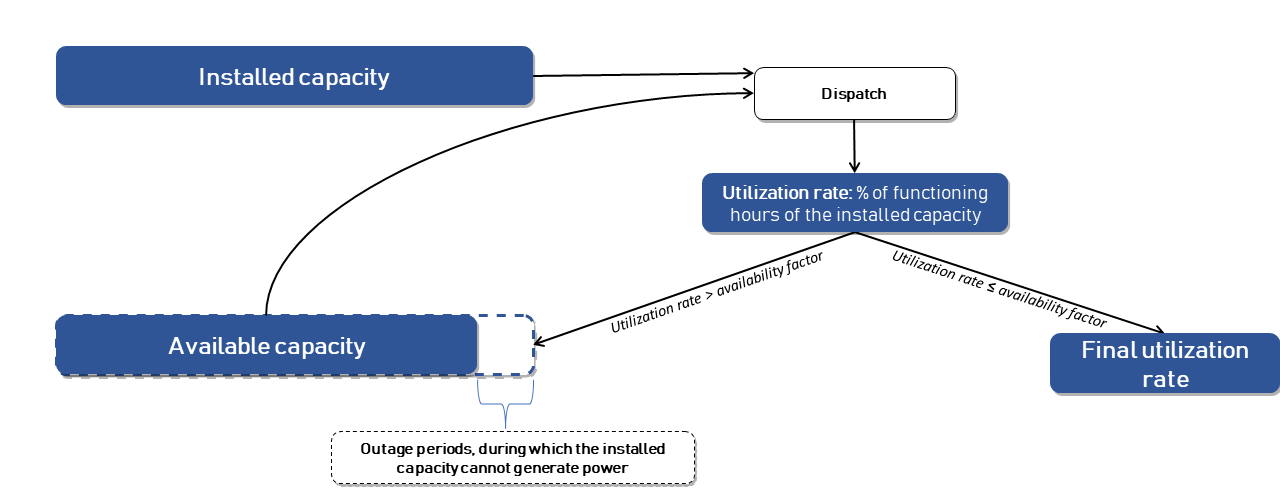
\includegraphics[scale=0.4]{figures&tables/availb.png}}
    \caption{Installed and available capacity during dispatch}
    \label{fig:avail}
\end{figure}


This production cost minimization program allows associating an average annual utilization period (in hours) in each region $k$ and for each technology. For conventional technologies, the utilization rate (the average functioning time of the installed capacity over the 8760 hours of the year) cannot exceed the availability factor. When this occurs for some technologies (e.g. coal units would run 100\% of the time according to the dispatch procedure, while their availability factor is 85\%), we introduce an available capacity variable to account for outages and maintenance, and perform the dispatch again as shown on Figure \ref{fig:avail}.

For conventional technologies using fossil fuels, the fuel consumption associated to the electricity produced is calculated directly from the average energy efficiency of electricity generation of the installed capacity of the technology.

\section{Linkage between the electricity sector and the rest of the economy}

The linkage between the electricity module and the macroeconomic core of IMACLIM-R covers
\begin{itemize}
    \item flowing from the macroeconomic core to the electricity sector, as inputs to the nexus : current electricity demand and fossil fuel prices
    \item after the investment and dispatch decisions, bottom-up information from the nexus: the price of electricity and input-output coefficients associated with electricity production, the new stock of capital in the electricity sector and its associated maximum level of physical output achievable ($Cap_{k}$).
\end{itemize}

The input part is straightforward and covered in section 4. The bottom-up information from the nexus serves as building blocks for the electricity sector supply curve. The shape of the supply curve determines the market clearing conditions and thus the final electricity price. The supply curve in the electricity sector (precisely, the inverse supply curve), as any sector of IMACLIM-R, can be interpreted as the sum of a marginal production cost plus a sector, region-specific markup for profits. Unless otherwise stated, perfect competition is assumed in the electricity sector. Thus, the markup only covers the costs related to investment and capital depreciation.
The marginal cost of electricity generation in region $k$ is given by:

\begin{dmath}
    Cm_{k} = \sum_{j}{}pIC_{j,k}*IC_{j,k} + (\Omega_{k}*w_{k})*l_{k}*(1+tax_{k}^{w})
    \label{eqn:Cm}
\end{dmath}

\begin{itemize}
    \item The technical unitary coefficients of production which characterize the electricity sector (quantities of different fuels required to produce a unit of electricity) are determined for coal, gas and liquid fuels ($tech = [coal,gas,et]$) by equation \ref{eqn:IC}.
\end{itemize}


\begin{dmath}
    IC_{tech,elec,k} = \frac{\frac{prod\_elec\_techno_{tech,k}}{rho\_elec_{tech,k}}}{Q\_elec}
    \label{eqn:IC}
\end{dmath}

\begin{itemize}
    \item The marginal cost is increasing with the level of electricity generation through the utilization rate $\Omega_{k} = \frac{Q_{k}}{Cap_{k}}$. Static decreasing returns are assumed in every sector of IMACLIM-R and are associated with lower labor productivity (see doc).
 %starting form here, we  write two versions: what is in the code and what is should look like
%current
%from what I get: we start from Qref which is assumed to be well calibrated using GTAP data
%then we suppose that at calibration year the capital stock in the elec sector => 80% utilization rate
%After that, at every period the initial maximum output increases by (sum(Cap_elec_MW_dep,'c')+sum(Inv_MW,'c'))./sum(Cap_elec_MWref,'c')

%ideal
 In the electricity sector $Cap_{k}$ is given by the stock of capital and the availability factor associated with the different installed electricity generation technologies.
\end{itemize}
\begin{dmath}
    Cap_{elec,k}(t) =  Cap\_elec\_MW_{k,j}(t)*Avail_\_factor_{k,j}(t)*full\_load\_hours
    \label{eqn:Cap}
\end{dmath}


The markup is fixed prior to market clearing. It is calibrated such that, at current intermediary and final prices, the sum of the average cost of electricity generation (including investment costs) and the markup equals the regional market price of electricity.


\section{Long-term projections for regional power systems}
In this section, we briefly present the key electricity nexus outputs from 2020 to 2100, namely production and installed capacity under two scenarios: a baseline scenario and a SSP2 scenario.

\newpage
\section{Annex}

\begin{figure}[H]
    \centering
    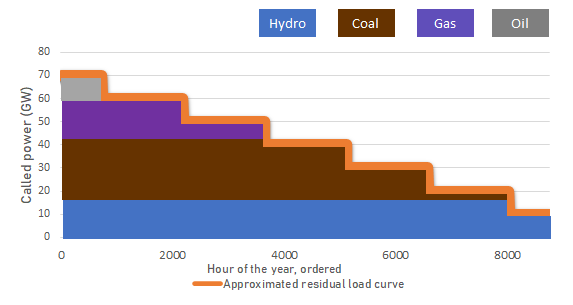
\includegraphics{figures&tables/dispatch.png}
    \caption{The merit order mechanism}
    \label{fig:dispatch}
\end{figure}

%the coef are given in the following order: (Intercept),Wind_share,PV_share,Wind_share_sq,PV_share_sq,Wind_share_cb,PV_share_cb,Wind_share:PV_share,PV_share:Wind_share_sq,Wind_share:PV_share_sq
    \begin{table}[H]
        \centering
        \begin{tabular}{|c||c|c|c|c|}
            \hline
                  & 1   & $x$ & $y$ \\
                  \hline
                  \hline
            1     &0.98&      & -1.003\\
            \hline
            $x$   & -0.242  &       & -1.653 \\
                  \hline
            $x^2$ & - 0.23    &  0.130     & 1.243 \\
            \hline
            $y^2$ &  0.945   &   1.224    &-0.422 \\
                  \hline
                  \hline
        \end{tabular}
        \caption{ coefficients for the $peak_{res}$ function (USA)}
    \end{table}
